\documentclass{ezb}
\usepackage[]{todonotes}
\usepackage{amsmath}
\usepackage{gensymb}
\usepackage{wrapfig}
\usepackage{longtable}
\usepackage{amssymb}
\usepackage{epstopdf}
\usepackage[colorlinks,        	% Links ohne Umrandungen in zu wählender Farbe
   linkcolor=black,   			% Farbe interner Verweise
   filecolor=black,   			% Farbe externer Verweise
   citecolor=black    			% Farbe von Zitaten
]{hyperref}
\usepackage{booktabs}

\renewcommand{\thesubsection}{\alph{subsection}}
\begin{document}

% \maketitle{Nummer}{Abgabedatum}{Tutor-Name}{Gruppennummer}
%           {Teilnehmer 1}{Teilnehmer 2}{Teilnehmer 3}
\maketitle{10.07.15}{Udo Frese}{1}{Annika Ofenloch - 2992807 - ofenloch@uni-bremen.de}{Frank Ihle - 3010158 - fihle@uni-bremen.de}{Simon Schirrmacher - 4000884 - simons@informatik.uni-bremen.de}{Noshaba Cheema - ncheema@uni-bremen.de}

%-------Text-Start------------------------------------------
\section{Harte Kante auf der Grafikkarte}
\begin{lstlisting}[language=C++]

__global__ void sobelKernel (uchar* dstImg, uchar* srcImg, int rows, int cols)
{
    //TODO: implement the sobel operator (6P)
	unsigned int x = blockDim.x * blockIdx.x + threadIdx.x;
	unsigned int y = blockDim.y * blockIdx.y + threadIdx.y;
	unsigned int step = gridDim.x * blockDim.x; 
	
	double sX = 0, sY = 0;
	
	if(in_img(x-1,y-1,rows,cols) && in_img(x+1,y+1,rows,cols)) {
		// (x,y) = step * y + x
		sX = (-srcImg[step * (y - 1) + x - 1] - 2 * srcImg[step * y + x - 1] - srcImg[step * (y + 1) + x - 1]
			 + srcImg[step * (y - 1) + x + 1] + 2 * srcImg[step * y + x + 1] + srcImg[step * (y + 1) + x + 1]) * 0.125;
			 
		sY = (-srcImg[step * (y - 1) + x - 1] - 2 * srcImg[step * (y - 1) + x] - srcImg[step * (y - 1) + x + 1]
			 + srcImg[step * (y + 1) + x - 1] + 2 * srcImg[step * (y + 1) + x] + srcImg[step * (y + 1) + x + 1]) * 0.125;
	}
	
	// save sobel length in image
	if(in_img(x,y,rows,cols))
		dstImg[step * y + x] = sqrt(sX * sX + sY * sY);
}

\end{lstlisting}
\begin{lstlisting}[language=C++]
void sobel (Mat_<uchar>& dstImg, const Mat_<uchar>& srcImg)
{
    //TODO: implement (4P)
	
	unsigned int data_length = dstImg.rows * dstImg.cols;
	size_t size = data_length * sizeof(uchar);
	
	uchar *gpuSrcImg, *gpuDstImg;
	
	// allocate memory for the images
	cudaMalloc((void**) &gpuSrcImg, size);
	cudaMalloc((void**) &gpuDstImg, size);
	
	// transfer the initialized source image to the device
	cudaMemcpy(gpuSrcImg, srcImg.data, size, cudaMemcpyHostToDevice);
	
	dim3 threads(16, 16);
	dim3 blocks(round_up(dstImg.cols, threads.x), round_up(dstImg.rows, threads.y));
	
	sobelKernel<<<blocks, threads>>>(gpuDstImg, gpuSrcImg, srcImg.rows, srcImg.cols);
	
	// copy results back to the host (implies cudaDeviceSynchronize())
	cudaMemcpy(dstImg.data, gpuDstImg, size, cudaMemcpyDeviceToHost);
	
	// free the memory
	cudaFree(gpuSrcImg);
	cudaFree(gpuDstImg);
	
	cudaDeviceReset();
}

\end{lstlisting}
\section{Schwarz und Weiß wir stehen an Eurer Seite}
Zu Beginn des Spieles und beim Anspiel nach einem Tor, werden die Roboter auf der Seite, welche ihrer Mannschaft entspricht, aufgestellt . Dadurch erfolgt die Zuordnung der Roboter zu der jeweiligen Mannschaft. Für den Algorithmus wird ein Partikelfilter eingesetzt, der vor allem dafür benutzt eine eindeutige Roboteridentifizierung zu ermöglichen.\\
\linebreak
Die Roboter müssen eine matte Oberfläche haben, damit Reflektionen vom Licht auf die schwarze Oberfläche der nicht als die weißen Kreise der Roboter identifiziert werden. Gleichermaßen empfiehlt es sich einen nicht reflektierenden Bodenbelag zu verwenden, so dass der Algorithmus nicht Reflektionen als Objekte erkennt.
\subsection{Filterbeschreibung}
Um jeden einzelnen Roboter zu verfolgen, wird für jeden Mannschafter einen unabhängigen Partikelfilter eingesetzt.
Für diese Filter ist die reale Position, die Geschwindigkeit und deren Richtung als Vektor des Roboters und die Gewichtung des Zustandes der Zustandsraum. Die Dynamikfuntion bildet mit Hilfe des vorherigen Zustands und den Fahrkommandos jedes einzelnen Roboters als Vektor einen neuen Zustand. Die Messfunktion gewichtet die einzelnen Zustände (Partikel) im Zustandsraum, wofür die Position des Roboters im Bild herangezogen wird. \\
\linebreak
Hierbei gehen wir davon aus, dass äußere Einflüsse, z.B. Kontakt mit anderen Robotern, welche die Position des Roboters beeinflussen, hinreichend gering und zufällig sind, dass diese als Messrauschen nicht weiter beachtet werden müssen.\\
\linebreak
Von dem Moment an, bei dem der Partikelfilter ein aussagekräftiges Ergebnis liefert, können die Mannschafter rückwirkend, identifiziert werden, in dem die Mannschaftsaufstellung dem Algorithmus mitgeteilt werden. Hierzu vergleicht er die Startposition auf der übermittelten Liste und seine berechnete Startposition. Alternativ kann die Identifizierung auch manuell vom Benutzer eingegeben werden, so ist die Roboteridentifikation von anfang an verfügbar.\\
\linebreak
Der Ball kann eindeutig von den Kreisen auf den Robotern unterschieden werden, da er nicht vor schwarzen Hintergrund liegt (hierfür gilt die Bedingung, dass die Spielfläche nicht schwarz ist).\\
\linebreak
\subsection{Sonderfälle}
Sollte es dazu kommen, dass ein Roboter nicht mehr im Bild erfasst werden kann (z.B. beim Umkippen oder er befindet sich außerhalb des Spielfeldes), wird der Partikelfilter neu initialisiert, sobald der Roboter wieder erfasst wird. Dieses Vorgehen funktioniert nur, wenn nur ein Roboter zu einer Zeit nicht mehr erfassbar ist. Sobald mehr als ein Roboter nicht mehr erfassbar ist, ist es nicht mehr möglich diese zu unterscheiden, wenn sie wieder im Bild erfasst werden, da es nun mehrere Möglichkeiten gibt, welcher Partikelfilter zu welchem Roboter gehört.\\
\linebreak
Bei Spielunterbrechungen (z.B.: Foul, Roboter muss aufgerichtet werden, oder wenn generell ein Mensch das Spielfeld betritt, etc.)  wird hierfür die Aktualisierung des Filters solange angehalten, bis das Spiel fortgesetzt wird. Damit dieser nicht mit offensichtlich falschen Informationen arbeitet und falsche Werte berechnet.\\
\linebreak
Falls die genannten Positions- und Identifikationsmechanismen trotz allem falsche Werte liefern, bietet sich an den Benutzer für diesen Sonderfall eintragen zu lassen. Dies muss auch gemacht werden, wenn ein Filter zurückgesetzt wurde, da mitten im Spiel nicht mehr ohne weiteres die Roboter voneinander unterschieden werden können.
\subsection{Ballerkennung}
Über den Spielball erhaltet man keine gesonderten Informationen und kann daher die Position über eine Kreiserkennung (z.B.: mit Hough) der Bildaufnahmen erfassen. Der Ball unterscheidet sich von den Kreisen der Roboter in sofern, dass er sich nicht auf schwarzem Hintergrund befindet.\\
\linebreak
Theoretisch kann auch eine mittlere Geschwindigkeit des Balls, anhand zweier Bilder, durch die Bildrate und der Ballposition auf beiden Aufnahmen, errechnet werden (je nach Anwendung des Vision-Servers). Den Ball über einen Partikelfilter zu erfassen wird nicht empfohlen, da sich der Ball des öfteren \textit{sprunghaft} von einer Richtung, in eine völlig andere bewegt. Hierfür müsste der Filter bei jedem Richtungswechsel zurückgesetzt werden, um sinnvolle Ergebnisse zu erhalten, da der Wechsel beim Konter- oder Passspiel in relativ kurzer Zeit passiert.
%Über den Ball haben wir keine dynamischen Informationen, weshalb die Geschwindigkeit des Balls anhand der Positionen im Bild ermittelt wird, indem die zurückgelegte Strecken zwischen den Bildern berechnet wird. Nach einigen Einzelbildern können wir nun aus den Daten eine Dynamikfuntion herleiten, indem wir die Geschwindigkeit proportional zur Reibungskraft ändern.\\
%Sollte der Ball nicht mehr im Bild zu erkennen sein, da er aus dem Bildbereich gefolgen ist oder sich direkt über einem Roboter befindet und nicht von der Markierung des Roboters unterschieden werden kann, wird der Partikelfilter neu initialisiert, sobald der ball wieder erfasst wurde. Dies ist ohne Weiteres möglich, da der Ball im Normalfall immer eindeutig identifiziert werden kann.
\section{Hinterm Horizont gehts weiter}
Die Kamera nimmt von einem Flugzeug aus die Landebahn auf, wie es in Abbildung \ref{landebahnAufgBild} dargestellt ist. Hierbei erkennt das Bildverarbeitungssystem zwei Geraden, die die Landebahn bilden und parallel zueinander liegen. Der Abstand zwischen den Geraden ist bekannt. Die Kamera hat einen schrägen Blickwinkel auf die Landebahn, da ansonsten keine Landebahn im Blickfeld der Kamera wäre. Es ist demnach ein Fluchtpunkt vorhanden, der sich ermitteln lässt, indem der Schnittpunkt der Geraden ermittelt wird. Ein Fluchtpunkt kann sich hierbei auch außerhalb des Bildes befinden. Es müssen lediglich die Geraden vorhanden sein.

\begin{figure}[htbp]
	\centering
	\fbox{
		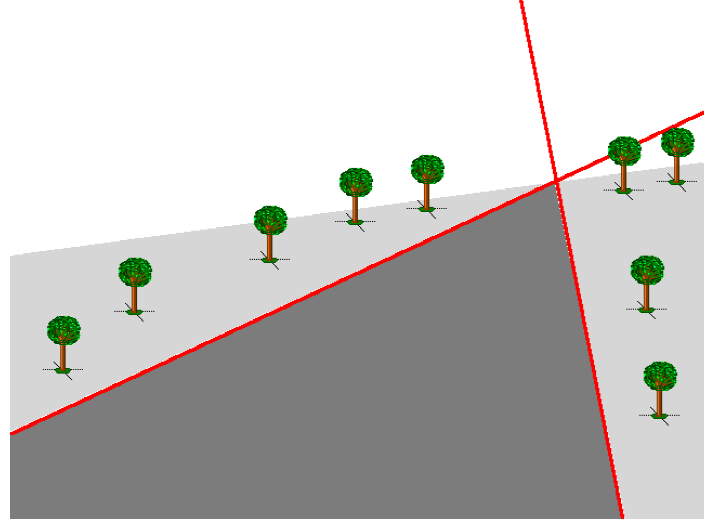
\includegraphics[scale=0.3]{landebahnAufgBild.png}
	}
	\caption{Landebahn mit Fluchtpunkt}
	\label{landebahnAufgBild}
\end{figure}

Eine Kamera verfügt über sechs Freiheitsgerade – die Translation in x-, y- und z-Richtung sowie die Rotation um die x mit dem Winkel $\alpha$, y mit dem Winkel $\beta$ und z Achse mit dem Winkel $\gamma$. Diese Kameraparameter beschreiben die Verschiebung  der Kamera zum Ursprung des Weltkoodinatensystems und die Drehung um die drei Euler Winkel. Es gibt jedoch einen Freiheitsgrad, der nicht beobachtet werden kann – die Translation in y-Richtung, wie es in der Abbildung \ref{yTranslation} zu sehen ist. Dies liegt daran, dass sich die Geraden (Landebahn) auf der Bodenebene (X,Y) liegen.

\begin{figure}[htbp]
	\centering
	\fbox{
		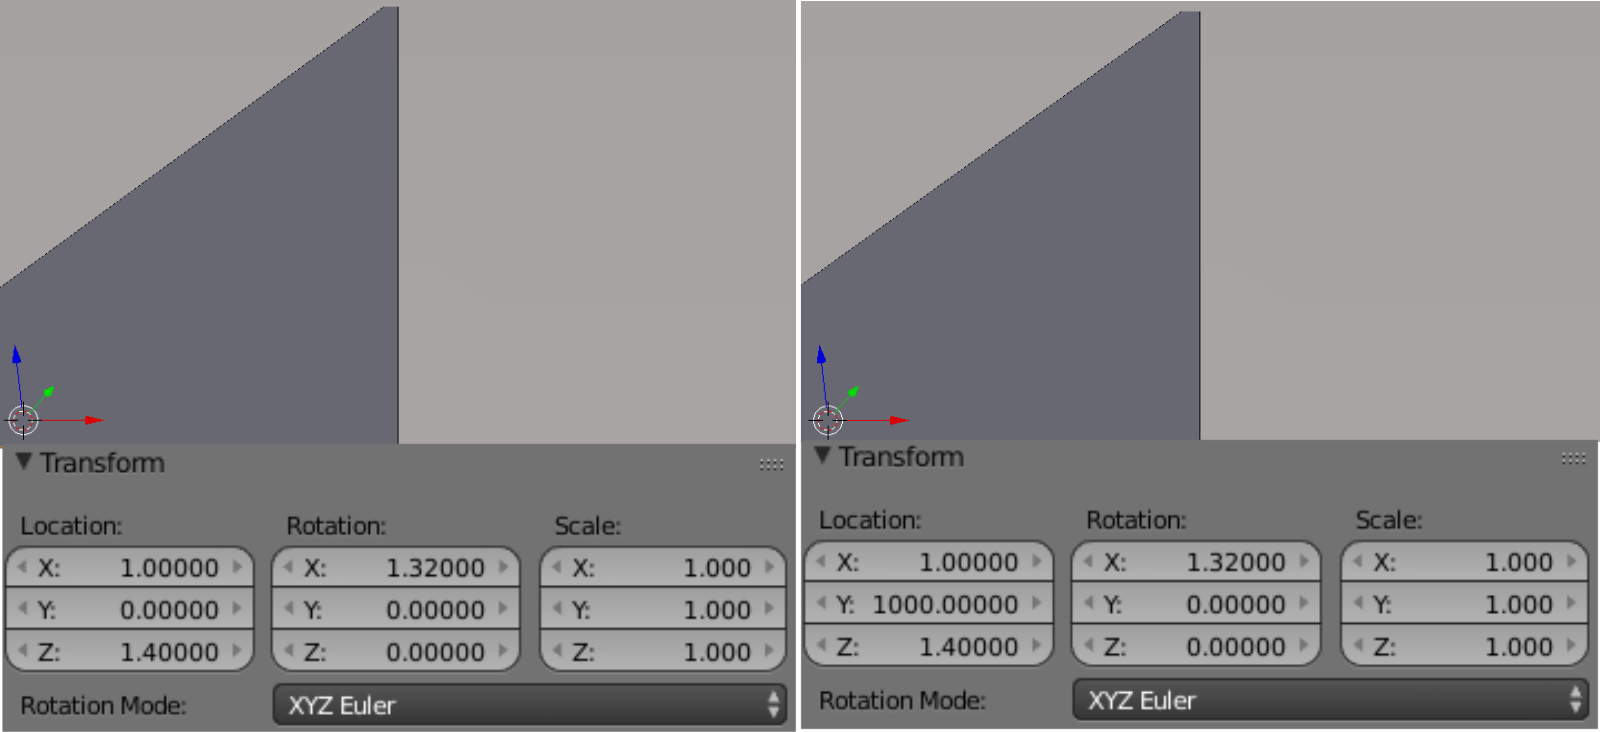
\includegraphics[scale=0.7]{yTranslation.png}
	}
	\caption{Links: Translation in y-Richtung = 0; Rechts: Translation in y-Richtung = 1000}
	\label{yTranslation}
\end{figure}

Ein Punkt $X$ mit den Koordinaten $(X,Y,Z)$ in der realen Welt hat einen korrespondierenden Punkt $x$ mit den Koordinaten $(u,v)$ auf der Bildebene. Die Punkte aus dem Raum (3D) können über die Projektionsmatrix $P$ in Punkte auf der Bildebene (2D) umgerechnet werden.

Die Projektionsmatrix hängt hierbei von den Orientierungsparametern ab. Die inneren Kameraparameter sind uns bekannt, da es sich in diesem Fall um eine kalibrierte Kamera handelt. Was wir benötigen, sind die äußeren Parameter der Kamera - die Lage der Kamera im Raum sowie die Blickrichtung der Kamera. Es muss demzufolge die Pose bestimmt werden.

Der Zusammenhang zwischen Objekt- und Bildpunkt lässt sich unter Verwendung der Projektionsmatrix, wie in der Matrizengleichung \ref{projectionmatrix} dargestellt, definieren.

\begin{equation} \label{projectionmatrix}
\begin{bmatrix}
u \\
v \\
w 
\end{bmatrix}
=
\begin{bmatrix}
p_{11} & p_{12} & p_{13} & p_{14} \\
p_{21} & p_{22} & p_{23} & p_{24} \\
p_{31} & p_{32} & p_{33} & p_{34} 
\end{bmatrix}
\begin{bmatrix}
X \\
Y \\
Z \\
W
\end{bmatrix}
\end{equation}  

Die Matrix $P$ hat 12 Einträge und 11 Freiheitsgrade, da der Skalierungsfaktor ignoriert werden kann. Theoretisch wird für das Lösen des Gleichungssystems 11 Gleichungen benötigt. In unserem Fall haben wir einige Annahmen und Vorgaben, die die Berechnung vereinfacht. Die Projektionsmatrix beinhaltet zum einen die Kalibrierungsmatrix und zum anderen die Rotationsmatrix. Da wir über die Kalibrieungsmatrix verfügen, besitzen wir bereits 5 Freiheitsgrade. Demnach fehlen nur noch die Freiheitsgrade für die Rotation (3 DOF) und Translation (3 DOF). Durch die Reduktion der Freiheitsgrade wäre es jetzt bereits möglich durch 3 bekannte Punkte die Lösungsmenge auf vier Lösungen zu reduzieren. Bei vier Punkten würde man eine eindeutige Lösung erhalten.

Wir können uns zur Vereinfachung einen weiteren Aspekt anschauen. Da die Landebahn auf der Bodenebene (X,Y) liegt, kann die z-Komponente ignoriert werden. Es führt zu einer singulären Lösungsmatrix. Mit Hilfe der Homographie kann die Projektionsmatrix sowie Rotation/Translation, falls die Kalibrierungsmatrix $K$ vorhanden ist, berechnet werden.

Die Homographie $H$ beschreibt die Abbildung zwischen zwei Flächen, in unserem Fall ist es die Landebahn. In der Gleichung \ref{homographie} ist die Definition dargestellt.

\begin{equation} \label{homographie}
\begin{bmatrix}
x_{'1} \\
x_{'2} \\
1 
\end{bmatrix}
=
\begin{bmatrix}
h_{11} & h_{12} & h_{13} \\
h_{21} & h_{22} & h_{23} \\
h_{31} & h_{32} & h_{33} 
\end{bmatrix}
\begin{bmatrix}
x_{1} \\
x_{2} \\
1 \\
\end{bmatrix}
\end{equation} 

Es wird nun angenommen, dass für die Fläche in der realen Welt $Z=0$ gilt. Demnach kann jeder Punkt wie folgt ausgedrückt werden: $P=(X, Y, 0, 1)^T$.
Die Projektionsmatrix ist definiert durch $P=K[R|t]$, wobei $t=-RC$ ist. $C$ stellt hierbei das Kameracenter dar. Die Abbildung zwischen 3D und 2D ist durch $x=PX$ definiert. Demzufolge lässt sich folgende Gleichung aufstellen:

\begin{equation}
x=PX=K
\begin{bmatrix}
r_{1} | r_{2} | r_{3} | t 
\end{bmatrix}
=
\begin{pmatrix}
X \\
Y \\
0 \\
1
\end{pmatrix}
\end{equation} 

Bei $r_{1}, r_{2}$ und $r_{3}$ handelt es sich um die erste, zweite und dritte Spalte der Rotationsmatrix. Da $Z=0$ ist, kommt man auf $r_{3} * Z = r_{3} * 0 = (0,0,0)^T$. Demzufolge kann $r_{3}$ für die folgende Betrachtung weggelassen werden (Es gilt $K[r_{1}|r_{2}|t] \approxeq H$):
\begin{equation}
K
\begin{bmatrix}
r_{1} | r_{2} | t 
\end{bmatrix}
\begin{pmatrix}
X \\
Y \\
1
\end{pmatrix}
=H
\begin{pmatrix}
X \\
Y \\
1
\end{pmatrix}
\end{equation} 

Wenn der Zusammenhang zwischen Objekt- und Bildpunkt bekannt ist, kann die Homographie über ein DLT berechnet werden. 

Zur Bestimmung der Rotationsmatrix $R$ und $t$ muss die Homographie $H$ zerlegt werden. Da $R$ orthogonal ist, gilt $r_3 = r_1 \times r_2$ und demnach folgende Gleichung:
\begin{equation}
P=K
\begin{bmatrix}
r_{1} | r_{2} | (r_1 \times r_2)| t 
\end{bmatrix}
\end{equation} 

Dadurch hat man alle Parameter, die die Informationen über die Kamera Pose bzw. Flugzeug Pose liefern. Es kann bei diesem Verfahren zu Abweichungen kommen, insbesondere, wenn die Kamera falsch kalibriert wurde.

[Vgl.\textit{Master-Arbeit: Entwicklung eines Augmented Reality
Frameworks auf Basis von Kamera-basierten
Trackingverfahren, Hendrik Brauer, 2010}]

% siehe Ansatz zur Posenbestimmung: http://userpages.uni-koblenz.de/~cg/Diplomarbeiten/DA_BernhardReinert.pdf

%-------Text-End------------------------------------------
\end{document}

